\subsection{RTKLIB interface}
    %Based on the rtkrcv commandline program from rtklib
    %Handles rtklib config and cmd files
    %Can play back log files as mentioned in section \ref{sec:imp:simulators}
    %

\subsection{Extended Kalman filter}
    %As described in section \ref{sec:imp:kalman}
    %PV estimation
    %Doppler, pseudorange
    %Describe tuning process (playback imc log?)
    
\begin{figure}
    \centering
    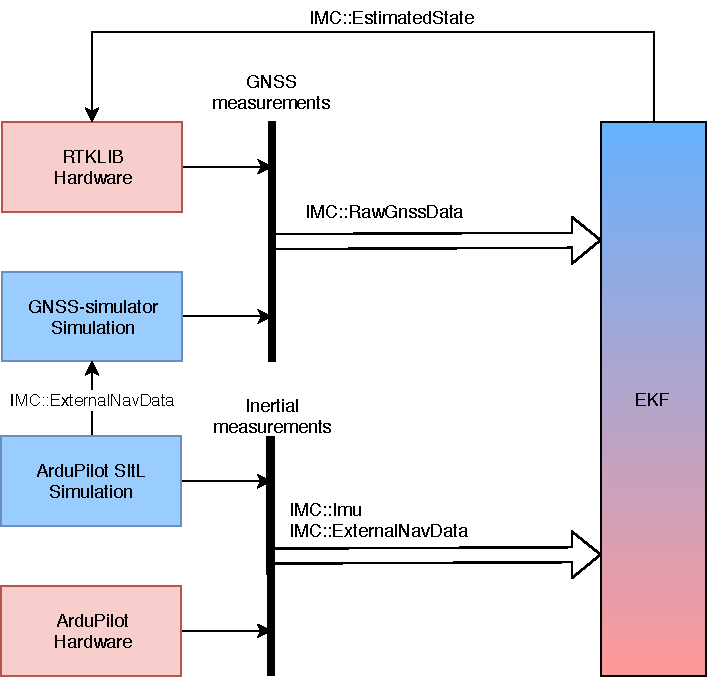
\includegraphics[scale=0.8]{Implementation/Images/dune-tasks.pdf}
    \caption{Overview of the EKF and the tasks it communicates with. Each box is a distinct task. The tasks are color coded as follows; The blue boxes are tasks used for the simulator, while the red ones runs on hardware. The EKF task depends only on the IMC-messages and runs with either profile.}
    \label{fig:dune-tasks}
\end{figure}